%% ----------------------------------------------------------------
%% Test.tex
%% ---------------------------------------------------------------- 

\chapter{Testing and Evaluation} \label{Chapter:Testing and Evaluation}

This chapter will provide information about the testing and evaluation process of this system. First of all, the functional testing will be carried out to identify whether this system meets the functional requirement specifications. Afterwards, the performance testing will be conducted to check whether the system performance affects the user experience. At last, this chapter will evaluate this system using a comparative survey and analyse the survey results.



\section{System Testing}

System testing is a crucial phase in the software development lifecycle because it ensures the software system can conform with all user requirements and achieve high quality. In this section, the black box testing will be conducted to test the functionalities of this system. Black box testing is a software testing process that verifies the functionalities and quality of the system without peering into its internal structure. 

\begin{table}[H]
\centering
\caption{Descriptions of Test Cases}
\label{my-label}
\begin{tabular}{|l|p{4cm}|p{8cm}|}
\hline
\textbf{ID} & \textbf{Test Scenario}                        & \textbf{Test Case}                                                               \\ \hline
TC-1        & Check search functionality                    & Check response on searching universities and courses                             \\ \hline
TC-2        & Check functionalities in ranking table part   & Check response on interacting with ranking table part                            \\ \hline
TC-3        & Check functionalities in course location part & Check response on interacting with the map in course location part               \\ \hline
TC-4        & Check functionalities in weather part         & Check response on interacting with the charts in weather part                    \\ \hline
TC-5        & Check functionalities in criminality part     & Check response on interacting with the map and the pie chart in criminality part \\ \hline
TC-6        & Check functionalities in infrastructure part  & Check response on interacting with the map in infrastructure part                \\ \hline
\end{tabular}
\end{table}

Therefore, the testing process only focuses on whether the actual outputs of this system match expectations, given certain input actions. Table 7.1 displays the test cases designed for this system with their descriptions, and Table 7.2 provides the results of test cases in the black box testing.

\begin{landscape}
\begin{center}
\begin{longtable}{|p{1cm}|p{3.5cm}|p{4cm}|p{3cm}|p{5cm}|p{2.5cm}|p{1cm}|}
\caption{Results of Black Box Testing} \label{tab:long} \\

\hline \multicolumn{1}{|c|}{\textbf{ID}}   &  \multicolumn{1}{|c|}{\textbf{Pre-conditions}}  &  \multicolumn{1}{|c|}{\textbf{Test Steps}}  &  \multicolumn{1}{|c|}{\textbf{Test Data}} &  \multicolumn{1}{|c|}{\textbf{Expected Results}} &  \multicolumn{1}{|c|}{\textbf{Actual Results}} &  \multicolumn{1}{|c|}{\textbf{Pass/Fail}} \\ \hline 
\endfirsthead

\multicolumn{7}{c}%
{{\bfseries \tablename\ \thetable{} -- continued from previous page}} \\
\hline \multicolumn{1}{|c|}{\textbf{ID}}  &  \multicolumn{1}{|c|}{\textbf{Pre-conditions}}  &  \multicolumn{1}{|c|}{\textbf{Test Steps}}  &  \multicolumn{1}{|c|}{\textbf{Test Data}} &  \multicolumn{1}{|c|}{\textbf{Expected Results}} &  \multicolumn{1}{|c|}{\textbf{Actual Results}} &  \multicolumn{1}{|c|}{\textbf{Pass/Fail}} \\ \hline 
\endhead

%\hline \multicolumn{7}{|r|}{{Continued on next page}} \\ \hline
\endfoot

%\hline \hline
%\endlastfoot

TC-1 & The users enter this website’s homepage & 1.Enter a university and a course \newline 2.Select from suggestions
 & University of Southampton, Computer Science & The webpage displays information about University of Southampton and Computer Science & As Expected & Pass \\ \hline
TC-2 &  The webpage displays the ranking table part & 1.Enter a university  \newline
2.Click the buttons in the table & University of Southampton & The ranking table shows the ranking information about University of Southampton & As Expected & Pass \\ \hline
TC-3 & The webpage displays the map in course location part & / & / & The map shows the location of University of Southampton and the geographic proximity and driving time from it to several metropolis & As Expected & Pass \\ \hline
TC-4 & The webpage displays the charts in weather part & 1.Click the legends below the charts  \newline
2.Hover over the lines or charts & / & The charts show the lines or bars and the tooltips about the weather in Southampton according to the test steps  & As Expected & Pass \\ \hline
TC-5 & The webpage displays the map in criminality part & 1.Select different months  \newline
2.Hover over the circles  & May 2016 & The map and pie chart display information about criminality in Southampton in May 2016 and the tooltips of different location & As Expected & Pass \\ \hline
TC-6 & The webpage displays the map in infrastructure part & 1.Select airport  \newline 2.Select train station
 & Airport, Train station & The map displays the location of airports and train stations in Southampton & As Expected & Pass \\ \hline



\end{longtable}
\end{center}
\end{landscape}

\section{System Evaluation}

System evaluation is a process of assessing the performance of a software system to identify whether it could be applied in the real world. This section will introduce a survey that was used for system evaluation and then analyse the results of the survey and the feedbacks from respondents.


\subsection{Survey Design
}

In order to evaluate this system, the comparative survey methodology was used to design the survey. Specifically, the survey aimed to compare this system with UCAS, an official website for international students to search for universities and courses in the UK, and identify the advantages and disadvantage of this system. In this survey, the respondents were firstly asked to complete several tasks in a task list. The aim of the task list was to help them understand how to use this system and compare it with UCAS by completing a list of tasks. Afterwards, the respondents were asked to complete the questionnaire hosted in iSurvey. The questionnaire consisted of four questions using the Likert scale, ranging from strongly disagree to strongly agree, and several open-ended questions to allow students give some feedbacks and further improvements about this system according to their experience in completing the task list. The task list and questionnaire were both sent to the respondents via emails. The task list and questionnaire can be found in Appendix B and Appendix C respectively.


\subsection{Results Analysis}


There were 17 respondents who took part in this survey and they are international students who planned to study in the UK for their higher education. Figure 7.1 shows most (82.4\%) of the respondents have previous experience in using websites like UCAS to search universities and courses for their higher education. 


\begin{figure}[H]
  \centering
  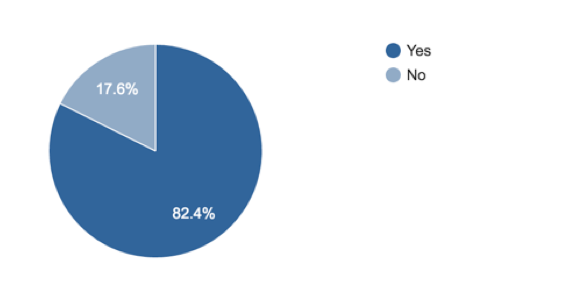
\includegraphics[width=10cm]{./img/Picture29}
  \caption{Previous Experience in Using Websites Like UCAS
}
  \label{Figure:figex}
\end{figure}


The following tables display the respondents’ opinions on this system from different aspects after completing the tasks in the task list. Table 7.3 shows most respondents agreed the user interface of this system were easy to learn and understand, and the user experience was good. However, some respondents thought some improvements should be considered in the user interface design and the user experience. Firstly, some of them complained that the loading time was a little bit long when they entered this system at the first time. Secondly, some respondents suggested that a back-to-top button could be added in the webpage to enable them to easily return to the search bar. Thirdly, some respondents pointed out that it was not convenient for them to compare several universities and cities at the same time and what they could do was searching and compare them over and over again. 


\begin{table}[H]
\centering
\caption{Opinions on the UI and UX
}
\label{my-label}
\begin{tabular}{|p{4cm}|c|c|c|c|c|c|c|}
\hline
                & \textbf{1} & \textbf{2} & \textbf{3} & \textbf{4} & \textbf{5} & \textbf{Weighted Mean} & \textbf{Interpretation} \\ \hline
User Interface  & 0          & 0          & 0          & 11         & 6          & 4.35                   & Agree                   \\ \hline
User Experience & 0          & 0          & 1          & 11         & 5          & 4.23                   & Agree                   \\ \hline
\end{tabular}
\end{table}


Table 7.4 shows the respondents’ opinions on the contents provided in this system. Most respondents strongly agreed that the contents provided in Course Location, Criminality and Infrastructure part were helpful for their destination choices.  The reason for this opinion was some of them thought course location, safety and infrastructure had great influences on their decision making for higher education, while others thought those contents could allow them to gain insights into universities from a different perspective. Some respondents thought the weather forecasts could give them a basic understanding of the weather in different cities, but it would more helpful if the historical information could be provided in this system. Moreover, some respondents hoped this system could provide some detailed descriptions about universities and courses in University\&Course part and some charts in Rakings Table part.

\begin{table}[H]
\centering
\caption{Opinions on Contents of This System}
\label{my-label}
\begin{tabular}{|p{4cm}|c|c|c|c|c|c|c|}
\hline
                   & \textbf{1} & \textbf{2} & \textbf{3} & \textbf{4} & \textbf{5} & \textbf{Weighted Mean} & \textbf{Interpretation} \\ \hline
University\&Course & 0          & 2          & 12         & 3          & 0          & 3.05                   & Neutral                 \\ \hline
Ranking Table      & 0          & 0          & 10         & 7          & 0          & 3.41                   & Neutral                 \\ \hline
Course Location    & 0          & 0          & 0          & 6          & 11         & 4.64                   & Strongly Agree          \\ \hline
Weather            & 0          & 1          & 4          & 7          & 5          & 3.94                   & Agree                   \\ \hline
Criminality        & 0          & 0          & 0          & 8          & 9          & 4.52                   & Strongly Agree          \\ \hline
Infrastructure     & 0          & 0          & 0          & 3          & 14         & 4.82                   & Strongly Agree          \\ \hline
\end{tabular}
\end{table}

Although this system has some shortcomings, most respondents agreed that this system was more helpful than UCAS (see Table 7.5), because they thought the information and visualisations provided in this system can provide comprehensive descriptions of universities and cities in the UK and help them make informed decisions. Besides, as shown in Figure 30, all of them were willing to recommend this system to their friends or peers if this system is applied in the real world. 

\begin{table}[H]
\centering
\caption{Comparison with UCAS
}
\label{my-label}
\begin{tabular}{|p{4cm}|c|c|c|c|c|c|c|}
\hline
                & \textbf{1} & \textbf{2} & \textbf{3} & \textbf{4} & \textbf{5} & \textbf{Weighted Mean} & \textbf{Interpretation} \\ \hline
More Helpful Than UCAS  & 0          & 0          & 1          & 10         & 6          & 4.29                   & Agree                   \\ \hline 
\end{tabular}
\end{table}


\begin{figure}[H]
  \centering
  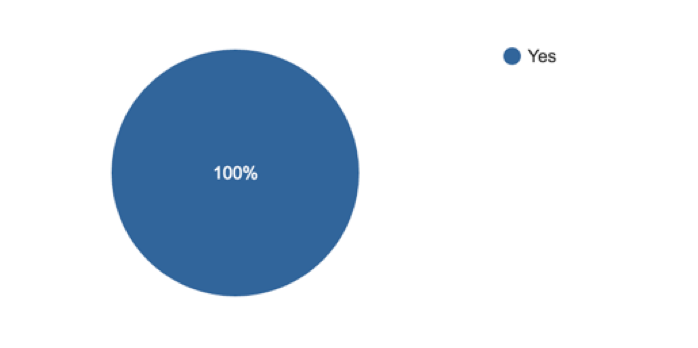
\includegraphics[width=11cm]{./img/Picture30}
  \caption{Willingness to Recommend This System
}
  \label{Figure:figex}
\end{figure}


\section{Summary}

This chapter introduces the testing and evaluation process of this system. The black box test is used to test the functionalities of this system, and the testing results proved that the functionalities of this system can work well and meet all user requirements. Besides, this system is evaluated using a comparative evaluation. Specially, a comparative survey containing a task list and an online questionnaire are used to compare this system with UCAS and gather the respondents’ opinions on this system. Though the results of evaluation show that this system has some shortcomings, the respondents thought this system helpful for international students’ destination choices in the UK.

